\section{Appendices} \label{sec:appendices}
% Test programs, test data, code, etc.
\subsection{Source Code}
\subsubsection{Main Function}
\lstinputlisting[language=Haskell]{../app/Main.hs}

\subsubsection{Main compiler}
\lstinputlisting[language=Haskell]{../src/Compiler.hs}

\subsubsection{Syntax}
\lstinputlisting[language=Haskell]{../src/Syntax.hs}

\subsubsection{Parser}
\lstinputlisting[language=Haskell]{../src/Parser.hs}

\subsubsection{Type Checker}
\lstinputlisting[language=Haskell]{../src/TypeCheckAnnotate.hs}

\subsubsection{AST Reversing}
\lstinputlisting[language=Haskell]{../src/AstReversing.hs}

\subsubsection{Evaluating Constant Expressions}
\lstinputlisting[language=Haskell]{../src/EvalExpr.hs}

\subsubsection{Optimizer}
\lstinputlisting[language=Haskell]{../src/AssertionRemoval.hs}

\subsubsection{AST Renaming}
\lstinputlisting[language=Haskell]{../src/RenameProcedures.hs}

\subsubsection{Procedure renmaing}
\lstinputlisting[language=Haskell]{../src/RenameProcedure.hs}

\subsubsection{\texttt{C++} Code Generation}
\lstinputlisting[language=Haskell]{../src/JapaToCpp.hs}

\subsection{Helper scripts and programs}

\subsubsection{Running tests}
\lstinputlisting[language=bash]{../bin/tester.sh}
\begin{figure}[H]
    \centering
    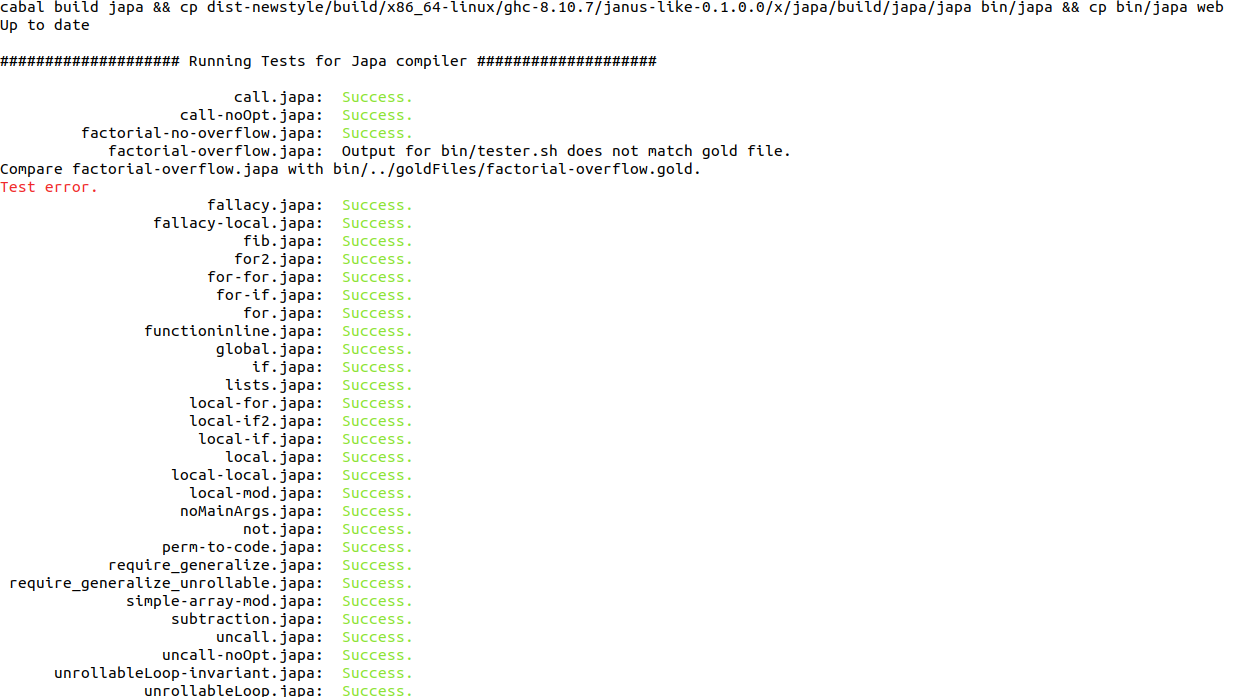
\includegraphics[scale=0.5]{imgs/testrun.png}
    \caption{A run through of the different gold file tests.}
    \label{fig:testrun}
\end{figure}

\subsubsection{Makefile}
\lstinputlisting[language=bash]{../Makefile}

\subsubsection{Benchmark script}
\lstinputlisting[language=Bash, label={lst:runbenchmark}]{../benchmarks/runbenchmark.sh}

\subsubsection{Benchmark compile time}
\lstinputlisting[language=Haskell]{../benchmarks/HaskellBenchmark.hs}

\subsubsection{Benchmark programs} \label{sec:benchmark-programs}
\lstinputlisting[language=c++]{../benchmarks/factorial.japa}
\lstinputlisting[language=c++]{../benchmarks/fib.japa}
\lstinputlisting[language=c++]{../benchmarks/perm-to-code.japa}

\subsection{Web interface}

\subsubsection{HTML index}
\lstinputlisting[language=HTML]{../web/index.html}

\subsubsection{Executing compiler}
\lstinputlisting[language=PHP]{../web/execute.php}

\subsubsection{Playground css}
\lstinputlisting[language=CSS]{../web/static/css/playground.css}

\subsubsection{Playground javascript}
\lstinputlisting[language=Javascript]{../web/static/js/playground.js}

\subsubsection{Playground text highlight}
\lstinputlisting[language=Javascript]{../web/static/js/ace/mode-janus.js}